\documentclass[a4paper, 12pt]{report}

%%%%%%%%%%%%
% Packages %
%%%%%%%%%%%%

\usepackage[english]{babel}
\usepackage[noheader]{packages/sleek}
\usepackage{packages/sleek-title}
\usepackage{packages/sleek-theorems}
\usepackage{packages/sleek-listings}

\usepackage{pgfplots}
\usepackage{tikz}
\usepackage{xcolor}
\usepackage{gensymb}

%%%%%%%%%%%%%%
% Title-page %
%%%%%%%%%%%%%%

\logo{./resources/img/NIT_Agartala_Logo.png}
\institute{National Institute of Technology\\Agartala}
% \faculty{Computer Science and Engineering}
\department{Department of Computer Science and Engineering}
\title{Digital Image Processing :}
\subtitle{A CONCEPT NOTE}
\author{\textit{Author}\\Jashaswimalya Acharjee\\Undergraduate Student, CSE Dept.}
\supervisor{\textit{Instructor}\\Dr. Parthasarathi De\\Assistant Professor, CSE Dept.}
%\context{Well, I was bored...}
\date{}

%%%%%%%%%%%%%%%%
% Bibliography %
%%%%%%%%%%%%%%%%

\addbibresource{./resources/bib/references.bib}

%%%%%%%%%%
% Others %
%%%%%%%%%%

\lstdefinestyle{latex}{
    language=TeX,
    style=default,
    %%%%%
    commentstyle=\ForestGreen,
    keywordstyle=\TrueBlue,
    stringstyle=\VeronicaPurple,
    emphstyle=\TrueBlue,
    %%%%%
    emph={LaTeX, usepackage, textit, textbf, textsc}
}

\FrameTBStyle{latex}

\def\tbs{\textbackslash}

%%%%%%%%%%%%
% Document %
%%%%%%%%%%%%

\begin{document}
    \maketitle
    \romantableofcontents

	\chapter{Introduction}

\section{Image}

An image is a two-dimensional function that represents a measure of some characteristics such as brightness or color of a viewed scene. An image is projection of a 3D scene into a 2D projection plane. It can be defined as a two-variable function $f(x,y)$ where for each position $(x,y)$ in the projection plane, $f(x,y)$ defines the light intensity at this point.

\subsection{Analog Image}

An Analog Image can be mathematically represented as a continuous range of values representing positions and intensity. An Analog Image is characterised by a physical magnitude varying continuously in space.

E.g.: The image produced on the screen of a CRT monitor is analog in nature.

\subsection{Digital Image}

A Digital Image is composed of picture elements called \textit{pixels}. Pixels are the smallest sample of an image. A pixel represents the brightness at one point. Conversion of an analog image into a digital image involves two important operations, namely, sampling and quantisation, which are illustrated in Fig: \ref{Digital-to-analog}.

\begin{figure}[h]
    \centering
\tikzset{every picture/.style={line width=0.75pt}} %set default line width to 0.75pt        

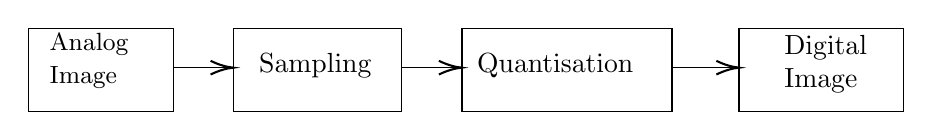
\begin{tikzpicture}[x=0.75pt,y=0.75pt,yscale=-1,xscale=1]
%uncomment if require: \path (0,300); %set diagram left start at 0, and has height of 300

%Shape: Rectangle [id:dp5271710061639749] 
\draw   (60,95) -- (129.8,95) -- (129.8,135) -- (60,135) -- cycle ;
%Shape: Rectangle [id:dp38336255974485245] 
\draw   (158.8,95) -- (239.8,95) -- (239.8,135) -- (158.8,135) -- cycle ;
%Shape: Rectangle [id:dp6224918178723147] 
\draw   (269,95) -- (370.16,95) -- (370.16,135) -- (269,135) -- cycle ;
%Shape: Rectangle [id:dp8433034035458677] 
\draw   (402.47,95) -- (481.8,95) -- (481.8,135) -- (402.47,135) -- cycle ;
%Straight Lines [id:da09940164773903648] 
\draw    (129.8,114) -- (156.8,114) ;
\draw [shift={(158.8,114)}, rotate = 180] [color={rgb, 255:red, 0; green, 0; blue, 0 }  ][line width=0.75]    (10.93,-3.29) .. controls (6.95,-1.4) and (3.31,-0.3) .. (0,0) .. controls (3.31,0.3) and (6.95,1.4) .. (10.93,3.29)   ;
%Straight Lines [id:da6636252308653761] 
\draw    (239.8,114) -- (266.8,114) ;
\draw [shift={(268.8,114)}, rotate = 180] [color={rgb, 255:red, 0; green, 0; blue, 0 }  ][line width=0.75]    (10.93,-3.29) .. controls (6.95,-1.4) and (3.31,-0.3) .. (0,0) .. controls (3.31,0.3) and (6.95,1.4) .. (10.93,3.29)   ;
%Straight Lines [id:da7001004518882727] 
\draw    (370.16,114) -- (400.47,114) ;
\draw [shift={(402.47,114)}, rotate = 180] [color={rgb, 255:red, 0; green, 0; blue, 0 }  ][line width=0.75]    (10.93,-3.29) .. controls (6.95,-1.4) and (3.31,-0.3) .. (0,0) .. controls (3.31,0.3) and (6.95,1.4) .. (10.93,3.29)   ;

% Text Node
\draw (69,96) node [anchor=north west][inner sep=0.75pt]   [align=left] {{\small Analog}\\{\small Image}};
% Text Node
\draw (170,106) node [anchor=north west][inner sep=0.75pt]   [align=left] {Sampling};
% Text Node
\draw (275,106) node [anchor=north west][inner sep=0.75pt]   [align=left] {Quantisation};
% Text Node
\draw (423.03,97) node [anchor=north west][inner sep=0.75pt]   [align=left] {Digital\\Image};

\end{tikzpicture}
\caption{Digital Image from Analog Image}
    \label{Digital-to-analog}
\end{figure}

\subsubsection{Advantages of Digital Images:}
The advantages of Digital Images are summarised below:
\begin{itemize}
    \item The Processing of images is faster and cost-effective.
    \item Digital Images can be effectively stored and efficiently transmitted from one place to another.
    \item When shooting a digital image, one can immediately see if the image is good or not.
    \item Copying a digital image is easy. The quality of digital image will not be degraded even if it is copied for several times.
    \item Whenever the image is in digital format, the reproduction of the image is both faster and cheaper.
    \item Digital technology offers plenty of scope for versatile image manipulation.
\end{itemize}

\subsubsection{Drawbacks of Digital Images:}
Some of the drawbacks of Digital Images are summarised below:
\begin{itemize}
    \item Misuse of copyright has become easier because images can be copied from Internet just by clicking the mouse a couple of times.
    \item A digital file cannot be enlarged beyond a certain size without compromising on quality.
    \item The memory required to store and process good-quality digital images is very high.
    \item For real-time implementation of digital-image-processing algorithms, the processor has to be very fast because the volume of data is very high.
\end{itemize}

\section{Digital Image Processing}

The processing of an image by means of a computer is generally termed as \textbf{Digital Image Processing}.

The Advantages of computers for the processing of images are summarised below:
\begin{itemize}
    \item \textbf{Flexibility and Adaptability:} The main advantage of digital computers when compared to analog electronic and optical information processing devices is that no hardware modifications are necessary in order to reprogram digital computers to solve different tasks. This feature makes digital computers an ideal devices for processing image signals adaptively.
    \item \textbf{Data Storage and Transmission:} With the development of different image-compression algorithms, the digital data can be effectively stored. The digital data within computers can be easily transmitted from one place to another.
\end{itemize}

The only limitation of Digital Image and Digital Image Processing are memory and processing speed capabilities of computers. Different Image-Processing techniques include \textit{Image Enhancements, image restoration, image fusion} and \textit{image watermarking}.

\section{Digital Image Representation}

A digital image is a two-dimensional discrete signal.
A digital image is also an $NxN$ array of elements.
Each element in the array is a number which represents the sampled intensity.
For e.g. : The representation of a $4x4$ image in matrix format is shown in Fig: \ref{matrix_view}.

\begin{figure}[h]
    
\begin{equation*}
    \begin{bmatrix}
    1 & 1 & 1 & 1\\
    1 & 1 & 1 & 1\\
    0 & 0 & 0 & 0\\
    0 & 0 & 0 & 0
    \end{bmatrix}
\end{equation*}

    \caption{Digital Image Representation}
    \label{matrix_view}
\end{figure}

Converting an image into a digital format can be done either with a digital camera, or by a scanner.
Digital images can be created directly on a computer screen.
However, it is restricted both in spatial coordinates (sampling) and in its allowed intensities (quantisation).

\subsection{Neighbours of a Pixel}
A pixel will have four neighbours if the neighbours exist in the EAST, WEST, NORTH and SOUTH directions. The four neighbours of the pixel `P' are represented in Fig: \ref{neighboursOfPixel}.

\begin{figure}[h]
    \centering

    \tikzset{every picture/.style={line width=0.75pt}} %set default line width to 0.75pt        

    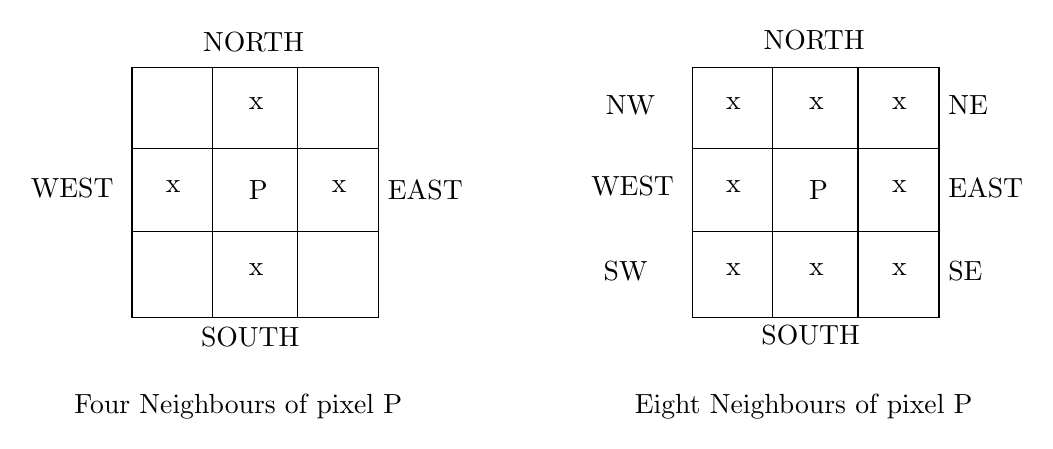
\begin{tikzpicture}[x=0.75pt,y=0.75pt,yscale=-1,xscale=1]
    %uncomment if require: \path (0,300); %set diagram left start at 0, and has height of 300
    
    %Shape: Rectangle [id:dp6330616545415024] 
    \draw   (51,51) -- (169.8,51) -- (169.8,171.2) -- (51,171.2) -- cycle ;
    %Shape: Rectangle [id:dp5493809441405086] 
    \draw   (51,90) -- (169.8,90) -- (169.8,130) -- (51,130) -- cycle ;
    %Shape: Rectangle [id:dp4349468061351809] 
    \draw   (89.8,51) -- (130.8,51) -- (130.8,171.2) -- (89.8,171.2) -- cycle ;
    
    %Shape: Rectangle [id:dp08063473849200564] 
    \draw   (321,51) -- (439.8,51) -- (439.8,171.2) -- (321,171.2) -- cycle ;
    %Shape: Rectangle [id:dp7254088029401085] 
    \draw   (321,90) -- (439.8,90) -- (439.8,130) -- (321,130) -- cycle ;
    %Shape: Rectangle [id:dp4119143208436029] 
    \draw   (359.8,51) -- (400.8,51) -- (400.8,171.2) -- (359.8,171.2) -- cycle ;
    
    
    % Text Node
    \draw (106,104) node [anchor=north west][inner sep=0.75pt]   [align=left] {P};
    % Text Node
    \draw (146,104) node [anchor=north west][inner sep=0.75pt]   [align=left] {x};
    % Text Node
    \draw (66,104) node [anchor=north west][inner sep=0.75pt]   [align=left] {x};
    % Text Node
    \draw (106,144) node [anchor=north west][inner sep=0.75pt]   [align=left] {x};
    % Text Node
    \draw (106,64) node [anchor=north west][inner sep=0.75pt]   [align=left] {x};
    % Text Node
    \draw (376,104) node [anchor=north west][inner sep=0.75pt]   [align=left] {P};
    % Text Node
    \draw (416,104) node [anchor=north west][inner sep=0.75pt]   [align=left] {x};
    % Text Node
    \draw (336,104) node [anchor=north west][inner sep=0.75pt]   [align=left] {x};
    % Text Node
    \draw (376,144) node [anchor=north west][inner sep=0.75pt]   [align=left] {x};
    % Text Node
    \draw (376,64) node [anchor=north west][inner sep=0.75pt]   [align=left] {x};
    % Text Node
    \draw (336,144) node [anchor=north west][inner sep=0.75pt]   [align=left] {x};
    % Text Node
    \draw (336,64) node [anchor=north west][inner sep=0.75pt]   [align=left] {x};
    % Text Node
    \draw (416,64) node [anchor=north west][inner sep=0.75pt]   [align=left] {x};
    % Text Node
    \draw (416,144) node [anchor=north west][inner sep=0.75pt]   [align=left] {x};
    % Text Node
    \draw (22,207) node [anchor=north west][inner sep=0.75pt]   [align=left] {Four Neighbours of pixel P};
    % Text Node
    \draw (292,207) node [anchor=north west][inner sep=0.75pt]   [align=left] {Eight Neighbours of pixel P};
    % Text Node
    \draw (1,103) node [anchor=north west][inner sep=0.75pt]   [align=left] {WEST};
    % Text Node
    \draw (83,175) node [anchor=north west][inner sep=0.75pt]   [align=left] {SOUTH};
    % Text Node
    \draw (173,104) node [anchor=north west][inner sep=0.75pt]   [align=left] {EAST};
    % Text Node
    \draw (84,33) node [anchor=north west][inner sep=0.75pt]   [align=left] {NORTH};
    % Text Node
    \draw (271,102) node [anchor=north west][inner sep=0.75pt]   [align=left] {WEST};
    % Text Node
    \draw (353,174) node [anchor=north west][inner sep=0.75pt]   [align=left] {SOUTH};
    % Text Node
    \draw (443,103) node [anchor=north west][inner sep=0.75pt]   [align=left] {EAST};
    % Text Node
    \draw (354,32) node [anchor=north west][inner sep=0.75pt]   [align=left] {NORTH};
    % Text Node
    \draw (443,143) node [anchor=north west][inner sep=0.75pt]   [align=left] {SE};
    % Text Node
    \draw (443,63) node [anchor=north west][inner sep=0.75pt]   [align=left] {NE};
    % Text Node
    \draw (278,63) node [anchor=north west][inner sep=0.75pt]   [align=left] {NW};
    % Text Node
    \draw (277,143) node [anchor=north west][inner sep=0.75pt]   [align=left] {SW};
    
    
    \end{tikzpicture}
    \caption{Neighbours of Pixels}
    \label{neighboursOfPixel}
\end{figure}

\section{Classification of Digital Images}

Digital Images can be broadly classified into two types and they are:
\begin{enumerate}
    \item Raster Image
    \item Vector Image
\end{enumerate}

\subsection{Raster Image or Bitmap Image}

\begin{itemize}
    \item A raster image file is generally defined as a rectangular array of regularly sampled values known as pixels.
    \item Scanned graphics and web graphics are the most common forms of raster images.
    \item Raster images are mapped to grids which are not easily scalable.
    \item A raster image is resolution dependent because it contains a fixed number of pixels that are used to create the image. Since there are a fixed and limited number of pixels, raster image will lose its quality if it is enlarged beyond that number of pixels as the computer will have to `make up' for the missing information.
    \item When an image is zoomed by a factory of 24 (say), the clarity is lost.
    \item Bitmaps are used for photorealistic images, and therefore, involve complex color variations.
    \item Raster images can show well the gradations of color and detailed images such as photographs.
    \item The spatial resolution of a raster image is determined by the resolution of the acquisition device and the quality of the original data source.
\end{itemize}

Common Raster Image formats include:
BMP (Windows Bitmap), PCX (Paintbrush), TIFF (Tag Interleave Format), JPEG/JPG (Join Photographics Expert Group), GIF (Graphics Interchange Format), PNG (Portable Network Graphics), PSD (Adobe Photoshop) and CPT (Corel PhotoPaint)

\subsection{Vector Image}

\begin{itemize}
    \item A vector image is defined by objects which are made of lines and curves that are mathematically defined in the computer.
    \item A vector can have various attributes such as line thickness, length and color.
    \item Vector images are mathematically defined and hence, they are scalable.
    \item This implies that vectors can be printed at any size, on any output device, at any resolution, without losing the detail and without altering the resultuion of the image.
    \item A Vector image, when zoomed by a factor of 24 (say), shows no distortion and clarity is preserved.
    \item Vector images can be scaled by several factors without altering the resolution of the image.
    \item Vector images are suitable for typography, line art and illustrations.
\end{itemize}

\section{Image Types}

Images can be broadly classified under four categories:
\begin{enumerate}
    \item Black \& White or Binary Image.
    \item Grayscale Image.
    \item Color Image.
    \item Multispectral Image.
\end{enumerate}

\subsection{Binary Image}
\begin{itemize}
    \item Binary Images take only two values, i.e. either `0' or `1'.
    \item The brightness graduation cannot be differentiated in Binary Images.
    \item A Grayscale image can be converted to Binary Image by the threshold operation.
    \item Geometric Properties of an object can be easily extracted from a binary image.
\end{itemize}

\subsection{Grayscale Image}
\begin{itemize}
    \item Grayscale images contain only brightness information.
    \item Each Pixel value in a grayscale image corresponds to an amount or quantity of light.
    \item The brightness graduation can be differentiated in a grayscale image.
    \item Each pixel is represented by a `byte' or` word'.
    \item An 8-bit image will have a brightness variation from 0 to 255 where `0' represents Black and `255' represents White.
\end{itemize}

\subsection{Color Image}
\begin{itemize}
    \item A color image has three values per pixel and they measure the intensity and chrominance of light.
    \item Each pixel is a vector of color components.
    \item Common Color spaces are RGB (Red, Green, Blue), HSV (Hue, Saturation, Value) and CMYK (Cyan, Magenta, Yellow, Black).
    \item The typical uncompressed data rate of a color image is three times the data rate of an uncompressed grayscale image.
\end{itemize}

\subsection{Volume Image}
\begin{itemize}
    \item A three-dimensional image is an example ofvolume image.
    \item The volume image can be optained from some medical imaging equipment in which the individual data points are called `voxels'.
    \item Voxel stands for Volume Pixel.
    \item A CAT Scan is an example of Volume Image.
\end{itemize}

\subsection{Range Image}

\begin{itemize}
    \item Range Images are a special class of digital images.
    \item Each pixel ofa range image expresses the distance between a known reference frame and a visible point in the screen.
    \item The range image reproduces the 3D structure of a scene.
    \item Range images are also referred as depth images.
\end{itemize}

\section{Image File Formats}

\begin{itemize}

    \item A digital image is often encoded in the form of binary files for the purpose of storage and transmission.
    \item A file format is a method used to store digital data and different file formats exist for storing images.
    \item Different file formats may compress the image data by differing amounts.
    \item Whatever be the format, the image file consists of two parts:
    \begin{enumerate}
        \item File Header
        \item Image Data
    \end{enumerate}
\end{itemize}

\subsubsection{Common Image File Formats:}

Various image file formats are widely used for the purpose fo digital storage and retrieval. Each of these file formats posses certain characteristics which makes them valid for various applications.
These include: GIF, JPEG/JPG, PNG, TIFF, PSD, EPS.

\subsection{File Header}

The Header part contains some of the vital information like format or version identification, width and height of the image, type of the image (binary, grayscale, color image) and image data format which specifies the order in which pixel values are stored in the image data section.
The header also specifies the type of compression mechanism.
The length of the File Header is often fixed.
The header information must provide all the necessary information to reconstruct the original data and its origanisation from the stored data.

\section{Applications of Digital Image Processing:}
Digital Image Processing is widely used in different fields like:
\begin{enumerate}
    \item Medicine
    \item Forensics
    \item Remote Sensing
    \item Communications
    \item Automobiles.
\end{enumerate}
	\cleardoublepage
	\chapter{Operations on Images}

\section{Pixel Connectivity}
The relationship between two or more pixels is defined as Pixel Connectivity.
Connectivity information is used to establish the boundaries of the objects.
The pixels $p$ and $q$ are said to be connected if certain conditions on pixel brightness specified by the set $V$ and spatial adjacency are satisfied.
For a binary image, this set $V$ will be $\{0,1\}$ and for grayscale images, $V$ might be of any range of Gray Levels.

\subsubsection{4-Connectivity:}
The pixels $p$ and $q$ are said to be in 4-connectivity when both have the same values as specified by the set $V$ and if $q$ is said to be in the set $N_4(p)$. This implies any path from $p$ to $q$ on which every other pixel is 4-connected to the next pixel.

In terms of pixel coordinates,
$$(x \pm 1, y) or (x, y \pm 1)$$

\subsubsection{6-Connectivity:}

6-connected pixels are neighbours to every pixel that touches one of their corners in a hexagonal grid or stretcher bond rectangular grid.
There are several ways to map hexagonal tiles to integer pixel coordinates.
With one method, in addition to the 4-connected pixels, the two additional pixel coordinates $$(x+1, y+1) and (x-1, y-1)$$ are connected to the pixel at $(x,y)$.

\subsubsection{8-Connectivity:}
It is assumed that the pixels $p$ and $q$ share a common grayscale value. The pixels $p$ and $q$ are said to be in 8-connectivity if $q$ is in the set $N_8(p)$.
In simpler terms, in addition to 4-connected pixels, each pixel with coordinates $$(x \pm 1, y \pm 1)$$ is connected to the pixel at $(x,y)$.
Eg: Fig: \ref{8-connectivity} shows 8-connectivity when $V = \{0,1\}$. Here, a multiple path or Loop is present.

\begin{figure}[h]
    \centering
    \tikzset{every picture/.style={line width=0.75pt}} %set default line width to 0.75pt        

    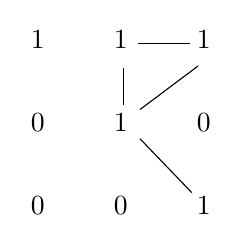
\begin{tikzpicture}[x=0.75pt,y=0.75pt,yscale=-1,xscale=1]
    %uncomment if require: \path (0,300); %set diagram left start at 0, and has height of 300

    %Straight Lines [id:da23478130696835353] 
    \draw    (77.8,45.2) -- (77.8,63.2) ;
    %Straight Lines [id:da8259417229972419] 
    \draw    (84.8,33.2) -- (109.8,33.2) ;
    %Straight Lines [id:da8853039395054243] 
    \draw    (85.8,65.2) -- (113.8,44.2) ;
    %Straight Lines [id:da02549560843434784] 
    \draw    (85.8,79.2) -- (110.8,105.2) ;

    % Text Node
    \draw (32,26) node [anchor=north west][inner sep=0.75pt]   [align=left] {1};
    % Text Node
    \draw (32,66) node [anchor=north west][inner sep=0.75pt]   [align=left] {0};
    % Text Node
    \draw (32,106) node [anchor=north west][inner sep=0.75pt]   [align=left] {0};
    % Text Node
    \draw (72,26) node [anchor=north west][inner sep=0.75pt]   [align=left] {1};
    % Text Node
    \draw (72,66) node [anchor=north west][inner sep=0.75pt]   [align=left] {1};
    % Text Node
    \draw (72,106) node [anchor=north west][inner sep=0.75pt]   [align=left] {0};
    % Text Node
    \draw (112,26) node [anchor=north west][inner sep=0.75pt]   [align=left] {1};
    % Text Node
    \draw (112,66) node [anchor=north west][inner sep=0.75pt]   [align=left] {0};
    % Text Node
    \draw (112,106) node [anchor=north west][inner sep=0.75pt]   [align=left] {1};

    \end{tikzpicture}

    \caption{8-Connectivity represented as lines}
    \label{8-connectivity}
\end{figure}

\subsubsection{Mixed Connectivity:}
Mixed Connectivity is also known as $m$-connectivity.
Two pixels $p$ and $q$ are said to be in $m$-connectivity when ---
\begin{enumerate}
    \item $q$ is in $N_4(p)$ or
    \item $q$ is in $N_D(p)$ and the intesection of $N_4(p)$ and $N_4(q)$ is empty.
\end{enumerate}

Eg: Fig: \ref{m-connectivity} shows an $m$-connectivity that there is no multiple paths or loops present in the connectivity. It can be observed that multiple paths have been removed.

\begin{figure}[h]
    \centering

    \tikzset{every picture/.style={line width=0.75pt}} %set default line width to 0.75pt        

    \begin{tikzpicture}[x=0.75pt,y=0.75pt,yscale=-1,xscale=1]
    %uncomment if require: \path (0,165); %set diagram left start at 0, and has height of 165
    
    %Straight Lines [id:da38565778933018646] 
    \draw    (207.8,45.2) -- (207.8,63.2) ;
    %Straight Lines [id:da331753409787636] 
    \draw    (214.8,33.2) -- (239.8,33.2) ;
    %Straight Lines [id:da5176626800362345] 
    \draw    (215.8,79.2) -- (240.8,105.2) ;
    
    % Text Node
    \draw (162,26) node [anchor=north west][inner sep=0.75pt]   [align=left] {1};
    % Text Node
    \draw (162,66) node [anchor=north west][inner sep=0.75pt]   [align=left] {0};
    % Text Node
    \draw (162,106) node [anchor=north west][inner sep=0.75pt]   [align=left] {0};
    % Text Node
    \draw (202,26) node [anchor=north west][inner sep=0.75pt]   [align=left] {1};
    % Text Node
    \draw (202,66) node [anchor=north west][inner sep=0.75pt]   [align=left] {1};
    % Text Node
    \draw (202,106) node [anchor=north west][inner sep=0.75pt]   [align=left] {0};
    % Text Node
    \draw (242,26) node [anchor=north west][inner sep=0.75pt]   [align=left] {1};
    % Text Node
    \draw (242,66) node [anchor=north west][inner sep=0.75pt]   [align=left] {0};
    % Text Node
    \draw (242,106) node [anchor=north west][inner sep=0.75pt]   [align=left] {1};
    
    \end{tikzpicture}

    \caption{$m$-connectivity}
    \label{m-connectivity}
\end{figure}

\section{Distance Measures}

The distance between the pixels $p$ and $q$ in an image can be given by distance measures such as Euclidean Distance, $D_4$ distance and $D_8$ distance.

Consider three pixels $p$,$q$ and $z$.
If the coordinates of the pixels are $P(x,y)$, $Q(s,t)$ and $Z(u,w)$ as shown in Fig: \ref{distanceSample}, the distances between the pixels can be calculated.

\begin{figure}[h]
    \centering

    \begin{equation*}
        \begin{matrix}
        0 & 1 & 1 & 1 & ( z)\\
        1 & 0 & 0 & 1 & \\
        1 & 1 & 1 & 1 & ( q)\\
        1 & 1 & 1 & 1 & \\
        ( p) &  &  &  & 
        \end{matrix}
    \end{equation*}

    \caption{Sample Image}
    \label{distanceSample}
\end{figure}

The distance function can be called \textit{Metric}, if the following properties are satisfied:
\begin{enumerate}
    \item $D(p,q)$ is well-defined and finite for all $p$ and $q$.
    \item $D(p,q) \geqslant 0$ if $p = q$, then $D(p,q)=0$.
    \item The distance $D(p,q) = D(q,p)$.
    \item $D(p,q) + D(q,z) \geqslant D(p,z)$. This is called property of triangular inequality.
\end{enumerate}

\subsubsection{Euclidean Distance:}
The Euclidean Distance between the pixels $p$ and $q$, with coordinates $(x,y)$ and $(s,t)$, respectively, can be defined as:
$$D_e(p,q) = \sqrt{(x-s)^2+(y-t)^2}$$
The advantage of Euclidean Distance is its simplicity.
However it is very computationally costly due to involvement of square root operations.

\subsubsection{$D_4$ Distance or City Block Distance:}
The $D_4$ distance or City Block Distance can be simply calculated as:
$$D_4(p,q) = |x-s| + |y-t|$$

\subsubsection{$D_8$ Distance or Chessboard Distance:}
This is calculated with the help of the following:
$$D_8(p,q) = \max (|x-s|, |y-t|)$$

\subsubsection{Question:}
Let $V = \{0,1\}$. Compute the $D_e$, $D_4$, $D_8$ and $D_m$ distances between two pixels $p$ and $q$. Let the pixel coordinates of $p$ and $q$ be $(3,0)$ and $(2,3)$ respectively, for the image shown below. Find the Distance Measures.

\begin{figure}[h]
    \centering

    \tikzset{every picture/.style={line width=0.75pt}} %set default line width to 0.75pt        

    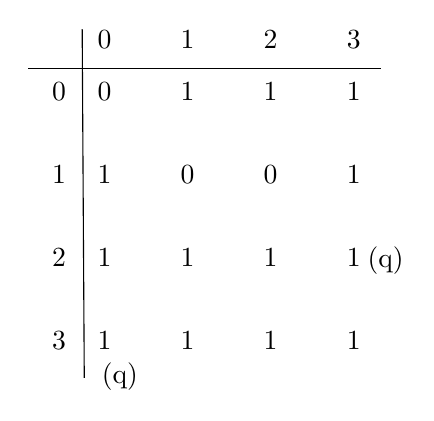
\begin{tikzpicture}[x=0.75pt,y=0.75pt,yscale=-1,xscale=1]
    %uncomment if require: \path (0,231); %set diagram left start at 0, and has height of 231
    
    %Straight Lines [id:da031132642263489663] 
    \draw    (19.8,40.4) -- (189.8,40.4) ;
    %Straight Lines [id:da9944079929840195] 
    \draw    (45.8,21.4) -- (46.8,189.4) ;
    
    % Text Node
    \draw (52,46) node [anchor=north west][inner sep=0.75pt]   [align=left] {0};
    % Text Node
    \draw (52,86) node [anchor=north west][inner sep=0.75pt]   [align=left] {1};
    % Text Node
    \draw (52,126) node [anchor=north west][inner sep=0.75pt]   [align=left] {1};
    % Text Node
    \draw (92,46) node [anchor=north west][inner sep=0.75pt]   [align=left] {1};
    % Text Node
    \draw (92,86) node [anchor=north west][inner sep=0.75pt]   [align=left] {0};
    % Text Node
    \draw (92,126) node [anchor=north west][inner sep=0.75pt]   [align=left] {1};
    % Text Node
    \draw (132,46) node [anchor=north west][inner sep=0.75pt]   [align=left] {1};
    % Text Node
    \draw (132,86) node [anchor=north west][inner sep=0.75pt]   [align=left] {0};
    % Text Node
    \draw (132,126) node [anchor=north west][inner sep=0.75pt]   [align=left] {1};
    % Text Node
    \draw (172,46) node [anchor=north west][inner sep=0.75pt]   [align=left] {1};
    % Text Node
    \draw (172,86) node [anchor=north west][inner sep=0.75pt]   [align=left] {1};
    % Text Node
    \draw (172,126) node [anchor=north west][inner sep=0.75pt]   [align=left] {1};
    % Text Node
    \draw (52,166) node [anchor=north west][inner sep=0.75pt]   [align=left] {1};
    % Text Node
    \draw (92,166) node [anchor=north west][inner sep=0.75pt]   [align=left] {1};
    % Text Node
    \draw (132,166) node [anchor=north west][inner sep=0.75pt]   [align=left] {1};
    % Text Node
    \draw (172,166) node [anchor=north west][inner sep=0.75pt]   [align=left] {1};
    % Text Node
    \draw (182,125) node [anchor=north west][inner sep=0.75pt]   [align=left] {(q)};
    % Text Node
    \draw (54,181) node [anchor=north west][inner sep=0.75pt]   [align=left] {(q)};
    % Text Node
    \draw (52,21) node [anchor=north west][inner sep=0.75pt]   [align=left] {0};
    % Text Node
    \draw (92,21) node [anchor=north west][inner sep=0.75pt]   [align=left] {1};
    % Text Node
    \draw (132,21) node [anchor=north west][inner sep=0.75pt]   [align=left] {2};
    % Text Node
    \draw (172,21) node [anchor=north west][inner sep=0.75pt]   [align=left] {3};
    % Text Node
    \draw (30,46) node [anchor=north west][inner sep=0.75pt]   [align=left] {0};
    % Text Node
    \draw (30,86) node [anchor=north west][inner sep=0.75pt]   [align=left] {1};
    % Text Node
    \draw (30,126) node [anchor=north west][inner sep=0.75pt]   [align=left] {2};
    % Text Node
    \draw (30,166) node [anchor=north west][inner sep=0.75pt]   [align=left] {3};
    
    \end{tikzpicture}

    \caption{Sample Image}
    \label{question3_1}
\end{figure}

\textbf{Solution:}\\

The Euclidean Distance is:

\begin{equation*}
    \begin{aligned}
    D_e & = \sqrt{( x-s)^{2} +( y-t)^{2}}\\
        & = \sqrt{( 3-2)^{2} +( 0-3)^{2}}\\
        & = \sqrt{1+9}\\
        & = \sqrt{10}
    \end{aligned}
\end{equation*}

\begin{equation*}
    \begin{aligned}
    D_4 & = \sqrt{|x-s| + |y-t|}\\
        & = |3-2| + |0-3|\\
        & = 1 + 3\\
        & = 4
    \end{aligned}
\end{equation*}

\begin{equation*}
    \begin{aligned}
    D_8 & = max(|x-s|, |y-t|)\\
        & = max(|3-2|, |0-3|)\\
        & = max(1,3)
    \end{aligned}
\end{equation*}

The distances can be checked with Fig: \ref{question3_abcd}.

The distance $D_m$ depends on the values of the set $V$. The implications of the set $V$ is that the path should be constructed only using the elements of $V$. So if the value of the set are changed, the path also changes.

The simplest $D_m$ distance can be calculated along the diagonal path. Here the distance is 3. Suppose the set $V = \{1\}$, the path of the distance $D_m$ also changes.

\begin{figure}[h]
    \centering


    \tikzset{every picture/.style={line width=0.75pt}} %set default line width to 0.75pt        

    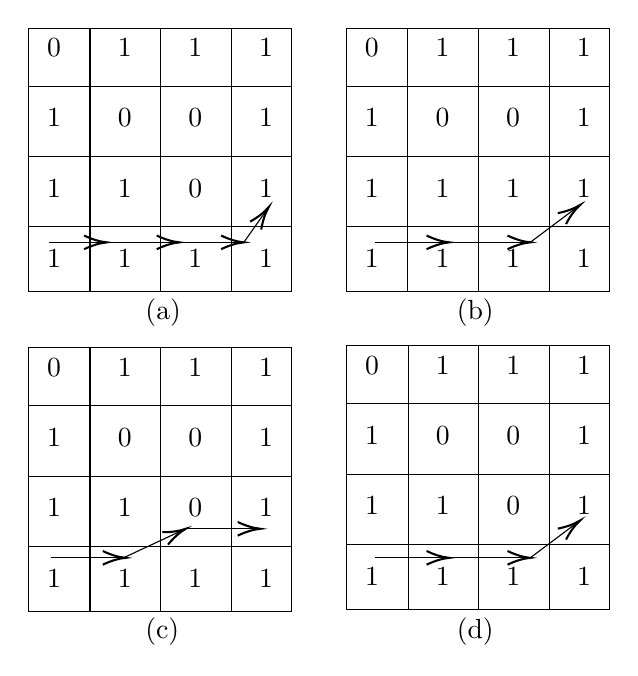
\begin{tikzpicture}[x=0.75pt,y=0.75pt,yscale=-1,xscale=1]
    %uncomment if require: \path (0,518); %set diagram left start at 0, and has height of 518
    
    %Shape: Rectangle [id:dp4475078963739587] 
    \draw   (40.97,18) -- (167.55,18) -- (167.55,145.03) -- (40.97,145.03) -- cycle ;
    %Straight Lines [id:da2837534659997365] 
    \draw    (70.57,18) -- (70.57,145.03) ;
    %Straight Lines [id:da08026350336095867] 
    \draw    (104.6,18) -- (104.6,145.03) ;
    %Straight Lines [id:da12341745735028331] 
    \draw    (138.63,18) -- (138.63,145.03) ;
    %Straight Lines [id:da18544345546390129] 
    \draw    (40.8,45.95) -- (167.55,45.95) ;
    %Straight Lines [id:da36332599792717035] 
    \draw    (40.8,79.82) -- (167.55,79.82) ;
    %Straight Lines [id:da24591625396036432] 
    \draw    (40.8,113.7) -- (167.55,113.7) ;
    %Shape: Rectangle [id:dp662906702606036] 
    \draw   (194.09,18) -- (320.68,18) -- (320.68,145.03) -- (194.09,145.03) -- cycle ;
    %Straight Lines [id:da12263567220380134] 
    \draw    (223.7,18) -- (223.7,145.03) ;
    %Straight Lines [id:da9762779391264798] 
    \draw    (257.73,18) -- (257.73,145.03) ;
    %Straight Lines [id:da8391602158100666] 
    \draw    (291.75,18) -- (291.75,145.03) ;
    %Straight Lines [id:da3444859343840154] 
    \draw    (193.92,45.95) -- (320.68,45.95) ;
    %Straight Lines [id:da09476418356870342] 
    \draw    (193.92,79.82) -- (320.68,79.82) ;
    %Straight Lines [id:da3655568500531654] 
    \draw    (193.92,113.7) -- (320.68,113.7) ;
    %Shape: Rectangle [id:dp8791357369590893] 
    \draw   (194.22,171) -- (320.8,171) -- (320.8,298.03) -- (194.22,298.03) -- cycle ;
    %Straight Lines [id:da05710193912163852] 
    \draw    (223.82,171) -- (223.82,298.03) ;
    %Straight Lines [id:da5717774023965383] 
    \draw    (257.85,171) -- (257.85,298.03) ;
    %Straight Lines [id:da25157700320628273] 
    \draw    (291.88,171) -- (291.88,298.03) ;
    %Straight Lines [id:da2995322489461316] 
    \draw    (194.05,198.95) -- (320.8,198.95) ;
    %Straight Lines [id:da6641804756632277] 
    \draw    (194.05,232.82) -- (320.8,232.82) ;
    %Straight Lines [id:da41797334591979096] 
    \draw    (194.05,266.7) -- (320.8,266.7) ;
    %Shape: Rectangle [id:dp4396916259579262] 
    \draw   (40.97,171.97) -- (167.55,171.97) -- (167.55,299) -- (40.97,299) -- cycle ;
    %Straight Lines [id:da052648741807676425] 
    \draw    (70.57,171.97) -- (70.57,299) ;
    %Straight Lines [id:da064462116667372] 
    \draw    (104.6,171.97) -- (104.6,299) ;
    %Straight Lines [id:da9610667135321806] 
    \draw    (138.63,171.97) -- (138.63,299) ;
    %Straight Lines [id:da384489478960784] 
    \draw    (40.8,199.92) -- (167.55,199.92) ;
    %Straight Lines [id:da9740468772342308] 
    \draw    (40.8,233.79) -- (167.55,233.79) ;
    %Straight Lines [id:da9410970713310336] 
    \draw    (40.8,267.67) -- (167.55,267.67) ;
    %Straight Lines [id:da4991960651404055] 
    \draw    (50.67,121.17) -- (76.67,121.17) ;
    \draw [shift={(78.67,121.17)}, rotate = 180] [color={rgb, 255:red, 0; green, 0; blue, 0 }  ][line width=0.75]    (10.93,-3.29) .. controls (6.95,-1.4) and (3.31,-0.3) .. (0,0) .. controls (3.31,0.3) and (6.95,1.4) .. (10.93,3.29)   ;
    %Straight Lines [id:da40533492288555495] 
    \draw    (77.67,121.17) -- (111.67,121.17) ;
    \draw [shift={(113.67,121.17)}, rotate = 180] [color={rgb, 255:red, 0; green, 0; blue, 0 }  ][line width=0.75]    (10.93,-3.29) .. controls (6.95,-1.4) and (3.31,-0.3) .. (0,0) .. controls (3.31,0.3) and (6.95,1.4) .. (10.93,3.29)   ;
    %Straight Lines [id:da5889055549592568] 
    \draw    (113.67,121.17) -- (142.67,121.17) ;
    \draw [shift={(144.67,121.17)}, rotate = 180] [color={rgb, 255:red, 0; green, 0; blue, 0 }  ][line width=0.75]    (10.93,-3.29) .. controls (6.95,-1.4) and (3.31,-0.3) .. (0,0) .. controls (3.31,0.3) and (6.95,1.4) .. (10.93,3.29)   ;
    %Straight Lines [id:da9582772307945706] 
    \draw    (144.67,121.17) -- (155.51,105.8) ;
    \draw [shift={(156.67,104.17)}, rotate = 485.22] [color={rgb, 255:red, 0; green, 0; blue, 0 }  ][line width=0.75]    (10.93,-3.29) .. controls (6.95,-1.4) and (3.31,-0.3) .. (0,0) .. controls (3.31,0.3) and (6.95,1.4) .. (10.93,3.29)   ;
    %Straight Lines [id:da23239242378169922] 
    \draw    (207.67,121.17) -- (241.67,121.17) ;
    \draw [shift={(243.67,121.17)}, rotate = 180] [color={rgb, 255:red, 0; green, 0; blue, 0 }  ][line width=0.75]    (10.93,-3.29) .. controls (6.95,-1.4) and (3.31,-0.3) .. (0,0) .. controls (3.31,0.3) and (6.95,1.4) .. (10.93,3.29)   ;
    %Straight Lines [id:da30210328263691966] 
    \draw    (243.67,121.17) -- (280.67,121.17) ;
    \draw [shift={(282.67,121.17)}, rotate = 180] [color={rgb, 255:red, 0; green, 0; blue, 0 }  ][line width=0.75]    (10.93,-3.29) .. controls (6.95,-1.4) and (3.31,-0.3) .. (0,0) .. controls (3.31,0.3) and (6.95,1.4) .. (10.93,3.29)   ;
    %Straight Lines [id:da27150216124144677] 
    \draw    (282.67,121.17) -- (305.07,104.37) ;
    \draw [shift={(306.67,103.17)}, rotate = 503.13] [color={rgb, 255:red, 0; green, 0; blue, 0 }  ][line width=0.75]    (10.93,-3.29) .. controls (6.95,-1.4) and (3.31,-0.3) .. (0,0) .. controls (3.31,0.3) and (6.95,1.4) .. (10.93,3.29)   ;
    %Straight Lines [id:da5600081587944892] 
    \draw    (207.67,273.17) -- (241.67,273.17) ;
    \draw [shift={(243.67,273.17)}, rotate = 180] [color={rgb, 255:red, 0; green, 0; blue, 0 }  ][line width=0.75]    (10.93,-3.29) .. controls (6.95,-1.4) and (3.31,-0.3) .. (0,0) .. controls (3.31,0.3) and (6.95,1.4) .. (10.93,3.29)   ;
    %Straight Lines [id:da07105978503613741] 
    \draw    (243.67,273.17) -- (280.67,273.17) ;
    \draw [shift={(282.67,273.17)}, rotate = 180] [color={rgb, 255:red, 0; green, 0; blue, 0 }  ][line width=0.75]    (10.93,-3.29) .. controls (6.95,-1.4) and (3.31,-0.3) .. (0,0) .. controls (3.31,0.3) and (6.95,1.4) .. (10.93,3.29)   ;
    %Straight Lines [id:da8864300844744744] 
    \draw    (282.67,273.17) -- (305.07,256.37) ;
    \draw [shift={(306.67,255.17)}, rotate = 503.13] [color={rgb, 255:red, 0; green, 0; blue, 0 }  ][line width=0.75]    (10.93,-3.29) .. controls (6.95,-1.4) and (3.31,-0.3) .. (0,0) .. controls (3.31,0.3) and (6.95,1.4) .. (10.93,3.29)   ;
    %Straight Lines [id:da03005048226319551] 
    \draw    (51.67,273.17) -- (85.67,273.17) ;
    \draw [shift={(87.67,273.17)}, rotate = 180] [color={rgb, 255:red, 0; green, 0; blue, 0 }  ][line width=0.75]    (10.93,-3.29) .. controls (6.95,-1.4) and (3.31,-0.3) .. (0,0) .. controls (3.31,0.3) and (6.95,1.4) .. (10.93,3.29)   ;
    %Straight Lines [id:da06389652649955102] 
    \draw    (116.67,259.17) -- (150.67,259.17) ;
    \draw [shift={(152.67,259.17)}, rotate = 180] [color={rgb, 255:red, 0; green, 0; blue, 0 }  ][line width=0.75]    (10.93,-3.29) .. controls (6.95,-1.4) and (3.31,-0.3) .. (0,0) .. controls (3.31,0.3) and (6.95,1.4) .. (10.93,3.29)   ;
    %Straight Lines [id:da3962475595082513] 
    \draw    (86.67,273.17) -- (114.85,260.01) ;
    \draw [shift={(116.67,259.17)}, rotate = 514.98] [color={rgb, 255:red, 0; green, 0; blue, 0 }  ][line width=0.75]    (10.93,-3.29) .. controls (6.95,-1.4) and (3.31,-0.3) .. (0,0) .. controls (3.31,0.3) and (6.95,1.4) .. (10.93,3.29)   ;
    
    % Text Node
    \draw (48.66,21.78) node [anchor=north west][inner sep=0.75pt]   [align=left] {0};
    % Text Node
    \draw (48.66,55.65) node [anchor=north west][inner sep=0.75pt]   [align=left] {1};
    % Text Node
    \draw (48.66,89.53) node [anchor=north west][inner sep=0.75pt]   [align=left] {1};
    % Text Node
    \draw (82.68,21.78) node [anchor=north west][inner sep=0.75pt]   [align=left] {1};
    % Text Node
    \draw (82.68,55.65) node [anchor=north west][inner sep=0.75pt]   [align=left] {0};
    % Text Node
    \draw (82.68,89.53) node [anchor=north west][inner sep=0.75pt]   [align=left] {1};
    % Text Node
    \draw (116.71,21.78) node [anchor=north west][inner sep=0.75pt]   [align=left] {1};
    % Text Node
    \draw (116.71,55.65) node [anchor=north west][inner sep=0.75pt]   [align=left] {0};
    % Text Node
    \draw (116.71,89.53) node [anchor=north west][inner sep=0.75pt]   [align=left] {0};
    % Text Node
    \draw (150.74,21.78) node [anchor=north west][inner sep=0.75pt]   [align=left] {1};
    % Text Node
    \draw (150.74,55.65) node [anchor=north west][inner sep=0.75pt]   [align=left] {1};
    % Text Node
    \draw (150.74,89.53) node [anchor=north west][inner sep=0.75pt]   [align=left] {1};
    % Text Node
    \draw (48.66,123.4) node [anchor=north west][inner sep=0.75pt]   [align=left] {1};
    % Text Node
    \draw (82.68,123.4) node [anchor=north west][inner sep=0.75pt]   [align=left] {1};
    % Text Node
    \draw (116.71,123.4) node [anchor=north west][inner sep=0.75pt]   [align=left] {1};
    % Text Node
    \draw (150.74,123.4) node [anchor=north west][inner sep=0.75pt]   [align=left] {1};
    % Text Node
    \draw (201.78,21.78) node [anchor=north west][inner sep=0.75pt]   [align=left] {0};
    % Text Node
    \draw (201.78,55.65) node [anchor=north west][inner sep=0.75pt]   [align=left] {1};
    % Text Node
    \draw (201.78,89.53) node [anchor=north west][inner sep=0.75pt]   [align=left] {1};
    % Text Node
    \draw (235.81,21.78) node [anchor=north west][inner sep=0.75pt]   [align=left] {1};
    % Text Node
    \draw (235.81,55.65) node [anchor=north west][inner sep=0.75pt]   [align=left] {0};
    % Text Node
    \draw (235.81,89.53) node [anchor=north west][inner sep=0.75pt]   [align=left] {1};
    % Text Node
    \draw (269.83,21.78) node [anchor=north west][inner sep=0.75pt]   [align=left] {1};
    % Text Node
    \draw (269.83,55.65) node [anchor=north west][inner sep=0.75pt]   [align=left] {0};
    % Text Node
    \draw (269.83,89.53) node [anchor=north west][inner sep=0.75pt]   [align=left] {1};
    % Text Node
    \draw (303.86,21.78) node [anchor=north west][inner sep=0.75pt]   [align=left] {1};
    % Text Node
    \draw (303.86,55.65) node [anchor=north west][inner sep=0.75pt]   [align=left] {1};
    % Text Node
    \draw (303.86,89.53) node [anchor=north west][inner sep=0.75pt]   [align=left] {1};
    % Text Node
    \draw (201.78,123.4) node [anchor=north west][inner sep=0.75pt]   [align=left] {1};
    % Text Node
    \draw (235.81,123.4) node [anchor=north west][inner sep=0.75pt]   [align=left] {1};
    % Text Node
    \draw (269.83,123.4) node [anchor=north west][inner sep=0.75pt]   [align=left] {1};
    % Text Node
    \draw (303.86,123.4) node [anchor=north west][inner sep=0.75pt]   [align=left] {1};
    % Text Node
    \draw (201.9,174.78) node [anchor=north west][inner sep=0.75pt]   [align=left] {0};
    % Text Node
    \draw (201.9,208.65) node [anchor=north west][inner sep=0.75pt]   [align=left] {1};
    % Text Node
    \draw (201.9,242.53) node [anchor=north west][inner sep=0.75pt]   [align=left] {1};
    % Text Node
    \draw (235.93,174.78) node [anchor=north west][inner sep=0.75pt]   [align=left] {1};
    % Text Node
    \draw (235.93,208.65) node [anchor=north west][inner sep=0.75pt]   [align=left] {0};
    % Text Node
    \draw (235.93,242.53) node [anchor=north west][inner sep=0.75pt]   [align=left] {1};
    % Text Node
    \draw (269.96,174.78) node [anchor=north west][inner sep=0.75pt]   [align=left] {1};
    % Text Node
    \draw (269.96,208.65) node [anchor=north west][inner sep=0.75pt]   [align=left] {0};
    % Text Node
    \draw (269.96,242.53) node [anchor=north west][inner sep=0.75pt]   [align=left] {0};
    % Text Node
    \draw (303.99,174.78) node [anchor=north west][inner sep=0.75pt]   [align=left] {1};
    % Text Node
    \draw (303.99,208.65) node [anchor=north west][inner sep=0.75pt]   [align=left] {1};
    % Text Node
    \draw (303.99,242.53) node [anchor=north west][inner sep=0.75pt]   [align=left] {1};
    % Text Node
    \draw (201.9,276.4) node [anchor=north west][inner sep=0.75pt]   [align=left] {1};
    % Text Node
    \draw (235.93,276.4) node [anchor=north west][inner sep=0.75pt]   [align=left] {1};
    % Text Node
    \draw (269.96,276.4) node [anchor=north west][inner sep=0.75pt]   [align=left] {1};
    % Text Node
    \draw (303.99,276.4) node [anchor=north west][inner sep=0.75pt]   [align=left] {1};
    % Text Node
    \draw (48.66,175.75) node [anchor=north west][inner sep=0.75pt]   [align=left] {0};
    % Text Node
    \draw (48.66,209.62) node [anchor=north west][inner sep=0.75pt]   [align=left] {1};
    % Text Node
    \draw (48.66,243.5) node [anchor=north west][inner sep=0.75pt]   [align=left] {1};
    % Text Node
    \draw (82.68,175.75) node [anchor=north west][inner sep=0.75pt]   [align=left] {1};
    % Text Node
    \draw (82.68,209.62) node [anchor=north west][inner sep=0.75pt]   [align=left] {0};
    % Text Node
    \draw (82.68,243.5) node [anchor=north west][inner sep=0.75pt]   [align=left] {1};
    % Text Node
    \draw (116.71,175.75) node [anchor=north west][inner sep=0.75pt]   [align=left] {1};
    % Text Node
    \draw (116.71,209.62) node [anchor=north west][inner sep=0.75pt]   [align=left] {0};
    % Text Node
    \draw (116.71,243.5) node [anchor=north west][inner sep=0.75pt]   [align=left] {0};
    % Text Node
    \draw (150.74,175.75) node [anchor=north west][inner sep=0.75pt]   [align=left] {1};
    % Text Node
    \draw (150.74,209.62) node [anchor=north west][inner sep=0.75pt]   [align=left] {1};
    % Text Node
    \draw (150.74,243.5) node [anchor=north west][inner sep=0.75pt]   [align=left] {1};
    % Text Node
    \draw (48.66,277.37) node [anchor=north west][inner sep=0.75pt]   [align=left] {1};
    % Text Node
    \draw (82.68,277.37) node [anchor=north west][inner sep=0.75pt]   [align=left] {1};
    % Text Node
    \draw (116.71,277.37) node [anchor=north west][inner sep=0.75pt]   [align=left] {1};
    % Text Node
    \draw (150.74,277.37) node [anchor=north west][inner sep=0.75pt]   [align=left] {1};
    % Text Node
    \draw (96,147) node [anchor=north west][inner sep=0.75pt]   [align=left] {(a)};
    % Text Node
    \draw (246,147) node [anchor=north west][inner sep=0.75pt]   [align=left] {(b)};
    % Text Node
    \draw (246,301) node [anchor=north west][inner sep=0.75pt]   [align=left] {(d)};
    % Text Node
    \draw (96,301) node [anchor=north west][inner sep=0.75pt]   [align=left] {(c)};
    
    
    \end{tikzpicture}
    
    \caption{Distance Measures: (a) Distance $D_e$, (b) Distance $D_4$ when $V=\{0,1\}$, (c) Distance $D_8$ when $V=\{0,1\}$, (d) Distance $D_m$ when $V=\{1\}$}
    \label{question3_abcd}
\end{figure}

	\cleardoublepage
	\chapter{Image Operations}

Image Operations are array operations.
These Operations are done on a pixel-by-pixel basis.
Array Operations are different from Matrix Operations.

Eg: Consider the two Images:
\begin{equation*}
    F_{1} \ =\ \begin{pmatrix}
    A & B\\
    C & D
    \end{pmatrix}
\end{equation*}
and
\begin{equation*}
    F_{2} \ =\ \begin{pmatrix}
    E & F\\
    G & H
    \end{pmatrix}
\end{equation*}

The multiplication of $F_1$ and $F_2$ is element-wise, as follows:

\begin{equation*}
    F_{1} \times F_{2}\ =\ \begin{pmatrix}
    AE & BF\\
    CG & DH
    \end{pmatrix}
\end{equation*}

In addition, one can observe that $F_1 \times F_2 = F_2 \times F_1$, whereas matrix multiplication is clearly different, since in matrices, $A \times B \neq B \times A$.
By default, image operations are array operations only.

\section{Arithmetic Operations}

Arithmetic operations include Image Addition, Subtraction, Multiplication, Division and Blending.

\subsection{Image Addition}

Two images can be added in a direct manner, as given by:
$$g(x,y) = f_1(x,y) + f_2(x,y)$$

The pixels of the input images $f_1(x,y)$ and $f_2(x,y)$ are added to obtain the resultant image $g(x,y)$.
However, it should be noted that the sum should not cross the allowed range for the datatype used.

Similarly it is possible to add any constant value to an image by:
$$g(x,y) = f_1(x,y) + k$$ where, $k$ is any constant.

If the value of $k$ is larger than 0, the overall `brightness' of the image is increased.

\textbf{Some Practical Applications of Image Addition:}
\subsubsection{Brightness of an image:}
The brightness of an image is the average pixel intensity of an image. If a positive or negative constant is added to all the pixels of an image, the average pixel intensity of the image increases or decreases, respectively. Thus adding a constant to all the pixels of an image increases its brightness and vice-versa. 

\subsubsection{Double Exposure:}
Double Exposure is the technique of superimposing an image on another image to produce the resultant. This gives the scenario equivalent to exposing a film to two pictures or Applying Watermarking on an image. This is done by adding One image on top of the other.

\subsection{Image Subtraction}

The Subtraction of two images can be done as follows:
$$g(x,y) = f_1(x,y) - f_2(x,y)$$
where, $f_1(x,y)$ and $f_2(x,y)$ are two input images and $g(x,y)$ is the output image.
To avoid negative values, it is desirable to find the modulus of the difference:
$$g(x,y) = |f_1(x,y) - f_2(x,y)|$$

It is also possible to subtract a constant value $k$ from the image, i.e. $g(x,y) = |f_1(x,y) - k|$, as $k$ is constant.
As discussed earlier, the decrease in the average intensity reduces the brightness of the image.

\textbf{Some practical applications of Image Subtraction are as follows:}
\begin{itemize}
    \item \textbf{Background Elimination:} This is done by subtracting the background image from the original image.
    \item \textbf{Brightness reduction:} This is done by subtracting a constant value from the whole image.
    \item \textbf{Change Detection:} This is done by subtracting two images and if the resultant value is non-zero, then there is a change between the two images.
\end{itemize}

\subsection{Image Multiplication}

Image Multiplication can be done in the following manner:
$$g(x,y) = f_1(x,y) \times f_2(x,y)$$
Here, $f_1(x,y)$ and $f_2(x,y)$ are two input images and $g(x,y)$ is the output image.

If the multiplied value crosses the maximum value of the data type of the images, the value of the pixel is reset to the maximum allowed value by that specific data type.

Similarly, scaling by a constant can be performed as:
$$g(x,y) = f(x,y) \times k$$
where, $k$ is a constant.

If $k$ is greater than 1, then the overall contrast increases.
If $k$ is less than 1, then the overall contrast decreases.


\textbf{NOTE:} The Brightness and Contrast can be manipulated together and also simulatneously by:
$$g(x,y) = a \times f(x,y) + k$$
Here, the parameters $a$ and $k$ are used to manipulate the contrast and brightness of the image $f(x,y)$ respectively, $g(x,y)$ is the output/resultant image.

\textbf{Some of the practical applications of Image Multiplication are as follows:}
\begin{itemize}
    \item \textbf{Manipulate Contrast:} If a fraction of $\geqslant$ 1 multiplied with the image, the overall contrast increases and vice-versa.
    \item \textbf{Filter Masks:} Useful for designing filter masks.
    \item \textbf{Highlighting AoI:} Used to create a mask to highlight area of interest.
\end{itemize}

\subsection{Image Division}

Similar to other previously discussed operations, the division operation can be performed in the following manner:
$$g(x,y) = \frac{f_1(x,y)}{f_2(x,y)}$$
where, $f_1(x,y)$ and $f_2(x,y)$ are the two input images and $g(x,y)$ is the output image.

Improper Data type specification may result in loss of information.

Division using a constant can also be performed, like:
$$g(x,y) = \frac{f(x,y)}{k}$$
where, $k$ is a constant.

\textbf{Some of the practical applications of Image Division are as follows:}
\begin{itemize}
    \item Change Detection.
    \item Separation of luminance and reflectance components.
    \item Contrast Reduction.
\end{itemize}

\section{Geometric Operations}
Let's discuss the Geometrical Operations used in Image Processing. These include: Translation, Scaling, Zooming, Linear Interpolation, Mirror or Reflection.

\subsection{Translation Operation}

Translation is the movement of an image to a new postion.
Let us assume that the point at the coordinate position $X = (x,y)$ of the matrix $F$ is moved to the new position $X'$ whose coordinate position is $(x',y')$.
Mathematically, this can be stated as a translation of a point $X$ to the new position $X'$.

This translation can be represented as:
\begin{gather*}
    x' = x + \delta x\\
    y' = y + \delta y
\end{gather*}

However, other transformations such as scaling and rotation are multiplicative in nature.
The transformation process for \textbf{rotation} is given by \textbf{$F' = RF$}, where \textbf{R} is the transform matrix for performing rotation.
Whereas, the transformation process for \textbf{scaling} is given by \textbf{$F' = SF$}. Here, \textbf{S} is the scaling transformation matrix.

To solve such a discrepancy and to create uniformity and consistency, it is necessary to use a homogeneous coordinate system where all transformations are treated as multiplications.
A point $(x,y)$ in 2D space is expressed as $(wx, wy, w)$ for $w \neq 0$.

The properties of homogeneous coordinates are as follows:
\begin{itemize}
    \item In homogeneous coordinates, at least one point should be non-zero. Thus $(0, 0, 0)$ does not exist in the homogeneous coordinate system.
    \item If one point is multiplicative of the other point, they are same. Thus, the points $(1, 3, 5)$ and $(3, 9, 15)$ are same as the second point is $3 \times (1, 3, 5)$.
    \item The point $(x, y, w)$ in the homogeneous coordinate system corresponds to the point $(\frac{x}{w}, \frac{y}{w})$ in 2D space.
\end{itemize}

Thus, in the homogeneous coordinate system, the translation process of the point $(x,y)$ to the new point $(x',y')$ of the image \textbf{$F$} is described as:
\begin{gather*}
    x' = x + \delta x\\
    y' = y + \delta y
\end{gather*}

In matrix form, this can be stated as:

\begin{equation*}
    \begin{bmatrix}
    x' & y' & 1
    \end{bmatrix}  = \begin{bmatrix}
    1 & 0 & \delta x\\
    0 & 1 & \delta y\\
    0 & 0 & 1
    \end{bmatrix}\begin{bmatrix}
    x & y & 1
    \end{bmatrix}^{T}
\end{equation*}

Sometimes, the image may not be present at the origin.
In that case, a suitable negative translational value can be used to bring the image to align with the origin.

\subsection{Scaling Operation}
Depending on the requirement, the object can be scaled.
\textit{Scaling} means enlarging and shrinking.
In the homogeneous coordinate system, the scaling of the point $(x,y)$ to the new point $(x',y')$ of the image \textbf{$F$} is described as:

\begin{gather*}
    x' = x \times S_x\\
    y' = y \times S_y
    \begin{bmatrix}
        x' & y'
    \end{bmatrix} = \begin{bmatrix}
        S_x & 0\\
        0 & S_y
    \end{bmatrix}\begin{bmatrix}
        x & y
    \end{bmatrix}
\end{gather*}

Here, $S_x$ and $S_y$ are called \textit{scaling factors} along $x$ and $y$ axes, respectively.
If the scaling factor is 1, then the object would appear larger.
If the scaling factors are fractions, the object would shrink.

\subsection{Zooming Operation}

The image can be zoomed using a process called pixel replication or interpolation.
Replication is called a zero-order hold process, where each pixel along the scan line is repeated once.
The the scan line is repeated.
The aim is to increase the number of pixels, thereby increasing the dimension of the image.

Eg: For the following image \textbf{$F$}:

\begin{equation}
    \begin{pmatrix}
        2 & 1\\
        1 & 3
    \end{pmatrix} = \begin{matrix}
        2 & 0 & 1 & 0\\
        0 & 0 & 0 & 0\\
        1 & 0 & 3 & 0\\
        0 & 0 & 0 & 0
    \end{matrix}
\end{equation}

This process is called \textbf{zero-order hold} process. Once 0s are inserted, the pixels are replicated to yield the following:

\begin{equation}
    \begin{matrix}
        2 & 2 & 1 & 1\\
        2 & 2 & 1 & 1\\
        1 & 1 & 3 & 3\\
        1 & 1 & 3 & 3
    \end{matrix}
\end{equation}

\subsection{Linear Interpolation Operation}

Consider the image:

\begin{equation*}
    H = \begin{pmatrix}
        2 & 1\\
        1 & 3
    \end{pmatrix}
\end{equation*}

Linear interpolation is equivalent to fitting a straight line by taking the average along the rows and columns.
The process is described as follows:
\begin{enumerate}
    \item For eg., the matrix $H$ can be zero-interlaced as:
        \begin{equation*}
            H = \begin{bmatrix}
                2 & 0 & 1 & 0\\
                0 & 0 & 0 & 0\\
                1 & 0 & 3 & 0\\
                0 & 0 & 0 & 0
            \end{bmatrix}
        \end{equation*}
    \item Interpolate the rows first. This is achieved by taking the average of the columns of that row. This yields:
        \begin{equation*}
            \begin{bmatrix}
                2 & 1.5 & 1 & 0.5\\
                0 & 0   & 0 & 0\\
                1 & 2   & 3 & 1.5\\
                0 & 0   & 0 & 0
            \end{bmatrix}
        \end{equation*}
    \item Interpolate Columns next. This is achieved by taking the average of the rows of that column. This yields:
        \begin{equation*}
            \begin{bmatrix}
                2   & 1.5  & 1   & 0.5\\
                1.5 & 1.75 & 2   & 1\\
                1   & 2    & 3   & 1.5\\
                0.5 & 1    & 1.5 & 0.75
            \end{bmatrix}
        \end{equation*}
\end{enumerate}

\subsection{Mirror or Reflection Operation}

This function creates the reflection of the object in a plane mirror. In other words, this function returns an image in which the pixels are reversed.
This operation is useful in creating an image in the desired order and for making comparisons.
The reflected object is of the same size as the original object, but the object is in the opposite quadrant.
Reflection is also described as rotation by $180\degree$.

The reflection along $x$-axis is given by:
$$F' = \begin{bmatrix}
    -x & y
\end{bmatrix} = \begin{bmatrix}
    1 & 0\\
    0 & -1
\end{bmatrix} \times \begin{bmatrix}
    x & y
\end{bmatrix}^{T}$$

Similarly, the reflection along the $y$-axis is given by:
$$F' = \begin{bmatrix}
    x & -y
\end{bmatrix} = \begin{bmatrix}
    -1 & 0\\
    0 & 1
\end{bmatrix} \times \begin{bmatrix}
    x & y
\end{bmatrix}^{T}$$

Similarly, the reflection along the $y = x$ is given by:
$$F' = \begin{bmatrix}
    x & -y
\end{bmatrix} = \begin{bmatrix}
    0 & 1\\
    1 & 0
\end{bmatrix} \times \begin{bmatrix}
    x & y
\end{bmatrix}^{T}$$

Similarly, the reflection along the $y=-x$ is given by:
$$F' = \begin{bmatrix}
    x & -y
\end{bmatrix} = \begin{bmatrix}
    0 & -1\\
    -1 & 0
\end{bmatrix} \times \begin{bmatrix}
    x & y
\end{bmatrix}^{T}$$


In homogeneous coordinate system, the matrices for reflection can be given as:
\begin{equation*}
    R_{y-axis} = \begin{bmatrix}
        -1 & 0 & 0\\
        0  & 1 & 0\\
        0  & 0 & 1
    \end{bmatrix} ;
    R_{x-axis} = \begin{bmatrix}
        1 & 0  & 0\\
        0 & -1 & 0\\
        0 & 0  & 1
    \end{bmatrix} ;
    R_{origin} = \begin{bmatrix}
        1 & 0 & 0\\
        0 & 1 & 0\\
        0 & 0 & -1
    \end{bmatrix}
\end{equation*}
	\cleardoublepage
    \chapter{Image Enhancement}

\section{Histogram Manipulation}

Histogram Manipulation basically modifies the histogram of an input image so as to improve the visual quality of the image.
In order to understand histogram manipulation, it is necessary to understand what a `Histogram' is and how `histogram equalisation' technique affects the visual quality of the image.

\subsection{Histogram}
The Histogram of an image is a plot or visual representation of the number of occurences of each gray level present in the image.
The Histogram provides a convenient summary of the intensities of an image, but it is unable to convey any information regarding spatial relationships between individual pixels.
The histogram provides more insight about image \textit{contrast} and \textit{brightness}.

Some properties of a typical histogram are listed as follows:
\begin{enumerate}
    \item The histogram of a dark image will be clustered towards the lower gray levels.
    \item The histogram of a bright image will be clustered towards the higher gray levels.
    \item For a low-contrast image, the histogram will not be spread equally, i.e., the histogram will be narrow.
    \item For a high-contrast image, the histogram will have an equal spread in the gray levels.
\end{enumerate}

The Image Brightness may be improved by modifying the histogram of the image.

\subsection{Histogram Equalisation}

Equalisation is a process that attempts to spread out the gray levels in an image so that they are evenly distributed across their range.
It flattens the histogram to create a better quality image.
Histogram equalisation reassigns the brightness values of pixels based on the image histogram.
Histogram equalisation is a technique where the histogram of the resultant image is as flat as possible.
It also provides a more visually pleasing result across a wider range of images.

\subsubsection{Procedure to Perform Histogram Equalisation:}

Histogram equalisation is done by performing the following steps:
\begin{enumerate}
    \item Create the frequency distribution table for each gray level from the given input image. 
    \item Find the running sum of the histogram values.
    \item Normalise the values from the previous step, by dividing by the total number of pixels.
    \item Multiply the values from the previous step, by the maximum gray-level value and round it to nearest integer.
    \item Map the gray level values to the result obtained in the previous step, using a one-to-one correspondence.
\end{enumerate}

\subsubsection{Question:}
Perform histogram equalisation of the following image.
\begin{equation*}
    \begin{bmatrix}
        4 & 4 & 4 & 4 & 4\\
        3 & 4 & 5 & 4 & 3\\
        3 & 5 & 5 & 5 & 3\\
        3 & 4 & 5 & 4 & 3\\
        4 & 4 & 4 & 4 & 4
    \end{bmatrix}
\end{equation*}

\textit{Solution:}\ \ \ \ The maximum value in this case is found to be 5.
A minimum of 3 bits to represent the number.
There are eight possible gray levels from 0 to 7.
The histogram of the input image is given below:

\begin{table}[h!]
    \centering
    \begin{tabular}{|c|c|c|c|c|c|c|c|c|}
        \hline
        Gray Level & 0 & 1 & 2 & 3 & 4 & 5 & 6 & 7\\
        \hline
        Number of Pixels & 0 & 0 & 0 & 6 & 14 & 5 & 0 & 0\\
        \hline
    \end{tabular}
\end{table}

\textbf\textit{Step 1:} Compute the running sum of histogram values.

\begin{table*}[h!]
    \centering
    \begin{tabular}{|c|c|c|c|c|c|c|c|c|}
        \hline
        Gray Level & 0 & 1 & 2 & 3 & 4 & 5 & 6 & 7\\
        \hline
        Number of Pixels & 0 & 0 & 0 & 6 & 14 & 5 & 0 & 0\\
        \hline
        Running Sum & 0 & 0 & 0 & 6 & 20 & 25 & 25 & 25\\
        \hline
    \end{tabular}
\end{table*}

\textbf\textit{Step 2:} Divide the Running Sum obtained in \textit{Step 1} by the total number of pixels. In this case, the total number of pixels is \textbf{25}.

\begin{table*}[h]
    \centering
    \begin{tabular}{|p{4.5cm}|c|c|c|c|c|c|c|c|}
        \hline
        Gray Level & 0 & 1 & 2 & 3 & 4 & 5 & 6 & 7\\
        \hline
        Number of Pixels & 0 & 0 & 0 & 6 & 14 & 5 & 0 & 0\\
        \hline
        Running Sum & 0 & 0 & 0 & 6 & 20 & 25 & 25 & 25\\
        \hline
        Running Sum / Total Number of Pixels & 0/25 & 0/25 & 0/25 & 6/25 & 20/25 & 25/25 & 25/25 & 25/25\\
        \hline
    \end{tabular}
\end{table*}

\textbf\textit{Step 3:} Multiply the result obtained in \textit{Step 2} by the maximum gray-level value, which is 7 in this case.

\begin{table*}[h]
    \centering
    \begin{tabular}{|p{4cm}|c|c|c|c|c|c|c|c|}
        \hline
        Gray Level & 0 & 1 & 2 & 3 & 4 & 5 & 6 & 7\\
        \hline
        Number of Pixels & 0 & 0 & 0 & 6 & 14 & 5 & 0 & 0\\
        \hline
        Running Sum & 0 & 0 & 0 & 6 & 20 & 25 & 25 & 25\\
        \hline
        Running Sum & 0 & 0 & 0 & 6 & 20 & 25 & 25 & 25\\
        \hline
        Multiplying by Maximum Gray Level & $\frac{0}{25}\times 7$ & $\frac{0}{25}\times 7$ & $\frac{0}{25}\times 7$ & $\frac{6}{25}\times 7$ & $\frac{20}{25}\times 7$ & $\frac{25}{25}\times 7$ & $\frac{25}{25}\times 7$ & $\frac{25}{25}\times 7$\\
        \hline
    \end{tabular}
\end{table*}

\textit{Rounding off to the closest Integer values.}

\begin{table*}[h]
    \centering
    \begin{tabular}{|c|c|c|c|c|c|c|c|c|}
        \hline
        Gray Level & 0 & 1 & 2 & 3 & 4 & 5 & 6 & 7\\
        \hline
        Number of Pixels & 0 & 0 & 0 & 6 & 14 & 5 & 0 & 0\\
        \hline
        Running Sum & 0 & 0 & 0 & 6 & 20 & 25 & 25 & 25\\
        \hline
        Running Sum & 0 & 0 & 0 & 6 & 20 & 25 & 25 & 25\\
        \hline
        Multiplying by Maximum Gray Level & 0 & 0 & 0 & 2 & 6 & 7 & 7 & 7\\
        \hline
    \end{tabular}
\end{table*}

\textbf\textit{Step 4:} Mapping of Gray Levels by one-to-one correspondence.

\begin{table*}[h]
    \centering
    \begin{tabular}{|c|c|}
        \hline
        Original Gray Level & Histogram Equalised Values\\
        \hline
        0 & 0\\
        \hline
        1 & 0\\
        \hline
        2 & 0\\
        \hline
        3 & 2\\
        \hline
        4 & 6\\
        \hline
        5 & 7\\
        \hline
        6 & 7\\
        \hline
        7 & 7\\
        \hline
    \end{tabular}
\end{table*}

Here, the Original Image and Histogram Equalised Image are shown side by side:

\begin{equation*}
    \centering
    \begin{bmatrix}
        4 & 4 & 4 & 4 & 4\\
        3 & 4 & 5 & 4 & 3\\
        3 & 5 & 5 & 5 & 3\\
        3 & 4 & 5 & 4 & 3\\
        4 & 4 & 4 & 4 & 4
    \end{bmatrix} \rightarrow \begin{bmatrix}
        6 & 6 & 6 & 6 & 6\\
        2 & 6 & 7 & 6 & 2\\
        2 & 7 & 7 & 7 & 2\\
        2 & 6 & 7 & 6 & 2\\
        6 & 6 & 6 & 6 & 6
    \end{bmatrix}
\end{equation*}

\section{Bit-Plane Slicing}

The Gray Level of each pixel in a digital image is stored as one or more bytes in a computer.
For an 8-bit image, 0 is encoded as 0 0 0 0 0 0 0 0, and 255 is encoded as 1 1 1 1 1 1 1 1.
Any Number between 0 and 255 is encoded as one byte.
The bit in the far left side is referred as the Most Significant Bit (MSB), because a change in that bit would significantly change the value encoded by the byte.
The bit in the far right is referred as the Least Significant Bit (LSB), because a change in this bit does not change the encoded gray value much.

Bit plane slicing is a method of representing an image with one or more bits of the byte used for each pixel.
One can use only the MSB to represent a pixel, which reduces the original gray level to a binary image.
The three main goals of bit plane slicing are:
\begin{enumerate}
    \item Converting a gray level image to a bianry image.
    \item Representing an image with fewer bits and compressing the image to a smaller size.
    \item Enhancing the image by focusing.
\end{enumerate}

\subsection{Bit-Plane Transformations}

It is possible to transform a gray level image into a sequence of binary images by taking advantage of its bit pattern storage.
For example, a gray level image is stored as an 8-bit image. Therefore, the image can be transformed into an 8-level image where the zero planes consist of the last bit of each gray level.
The first plane consists of the first bit of each gray value.
Similarly, the most significant bit plane has the greatest effect in terms of the magnitude of the image.
It is roughly equivalent to the threshold of the image at level 127.
Depending on the requirement, the bit planes can be retained or ignored.

\subsubsection{Question:}
Show the bit-plane slicing of the following image:
\begin{equation*}
    \begin{bmatrix}
        7 & 6 & 5\\
        4 & 3 & 2\\
        1 & 1 & 0
    \end{bmatrix}
\end{equation*}

\textit{Solution:}
The Binary Equivalent of the pixels is:

\begin{equation*}
    \begin{bmatrix}
        111 & 110 & 101\\
        100 & 011 & 010\\
        001 & 001 & 000
    \end{bmatrix}
\end{equation*}

\textit{Case-I:} When LSB is changed to 0, this image is reduced to:

\begin{equation*}
    \begin{bmatrix}
        110 & 110 & 100\\
        100 & 010 & 010\\
        000 & 000 & 000
    \end{bmatrix}
\end{equation*}

The Equivalent Image of the above:

\begin{equation*}
    \begin{bmatrix}
        6 & 6 & 4\\
        4 & 2 & 2\\
        0 & 0 & 0
    \end{bmatrix}
\end{equation*}

\textit{Case-II:} When the MSB is changed to 0, this image changes to:

\begin{equation*}
    \begin{bmatrix}
        011 & 010 & 001\\
        000 & 011 & 010\\
        001 & 001 & 000
    \end{bmatrix}
\end{equation*}

The Equivalent Image of the above Binary Image:

\begin{equation*}
    \begin{bmatrix}
        3 & 2 & 1\\
        0 & 3 & 2\\
        1 & 1 & 0
    \end{bmatrix}
\end{equation*}

Thus, Bit-Plane Slicing Leads to Transformation of Images.

\end{document}